\section{RISC-V}

\begin{figure}[H]
    \centering
    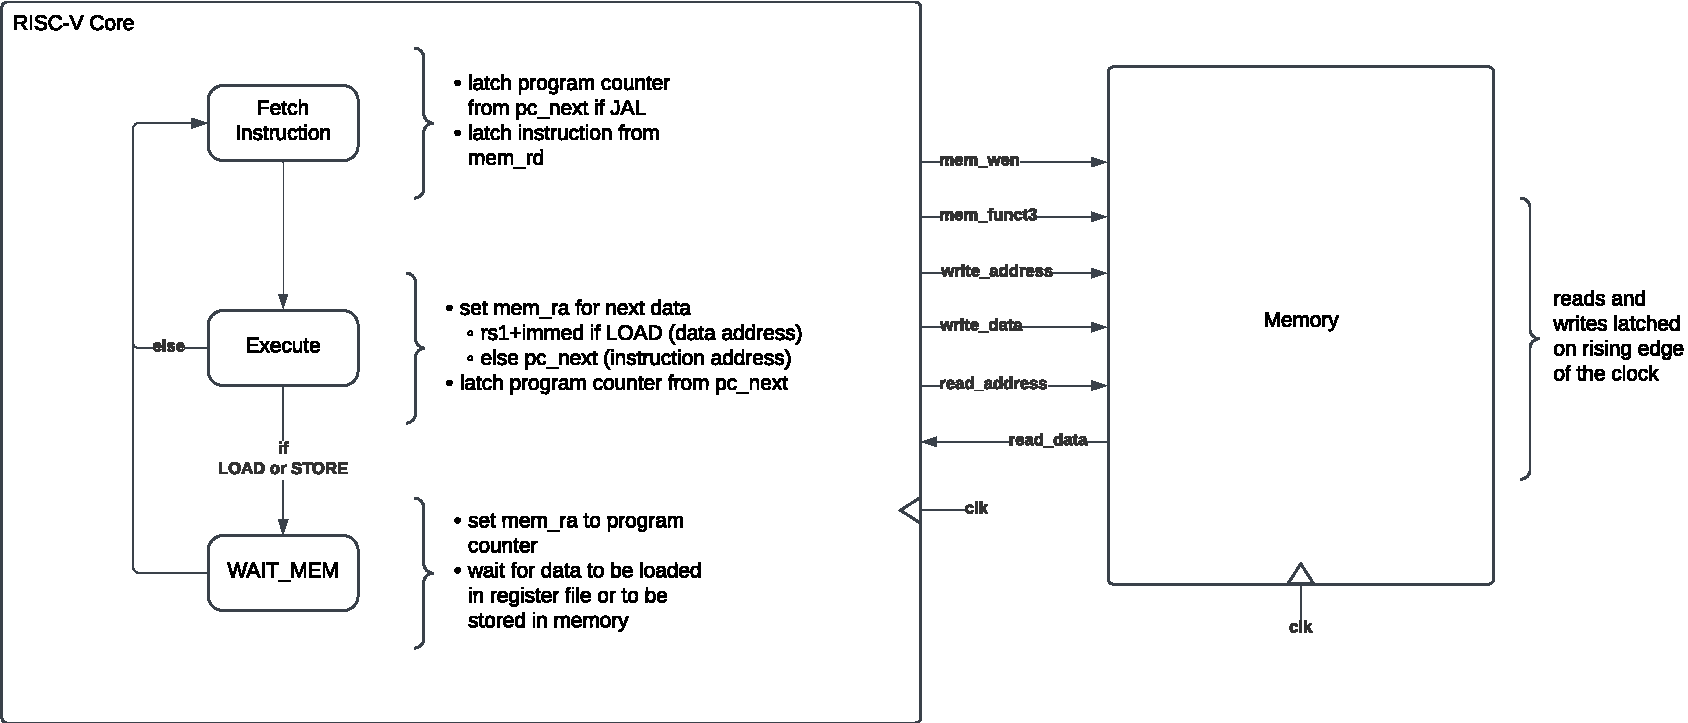
\includegraphics[width=\textwidth]{media/riscv}
    \caption{RISC-V processor connected to data and instruction memory}
    \label{fig:riscv}
\end{figure}

\subsection{State Machine}

The RISC-V processor operates as a finite state machine with three main states:
\begin{itemize}
\item
    \texttt{FETCH\_INSTR}:
        The processor fetches the next instruction from memory.
        If the previous instruction was a jump (JAL), the program counter is updated here.
        Otherwise, it proceeds to the execute phase.

\item
    \texttt{EXECUTE}:
        The processor performs computation or determines the next step based on the instruction type.
        If it’s a load or store instruction, the processor transitions to the \texttt{WAIT\_MEM} state to access memory.
        Otherwise, it immediately moves to the next instruction, usually after writing the results to the register file.

\item
    \texttt{WAIT\_MEM}:
        This state allows the processor to wait one cycle for memory to respond with the requested data (load) or acknowledge a store.
        Afterward, the state returns to \texttt{FETCH\_INSTR}.
\end{itemize}

These states control instruction sequencing, memory access timing, and ensure correct operation for instructions involving memory.
For all instructions except load and store, the processor completes the operation in two cycles, and three cycles otherwise.
This is possible because the processor latches the next instruction at the end of \texttt{EXECUTE} state and most signals are calculated combinationally.

\subsection{Top-Level Module}

The top module connects the RISC-V core to the memory module in Von Neumann architecture, where data and instructions live in the same place.
A system clock is generated either through simulation (\texttt{clk}) or by configuring a hardware oscillator and PLL to produce a 12\,MHz clock for the physical FPGA.
The RISC-V core sends memory read and write requests to the memory module based on the instruction.
The memory module responds to read and write requests synchronously, using the funct3 control signal.
The memory module also maps onboard LEDs (\texttt{LED}, \texttt{RGB\_R}, \texttt{RGB\_G}, \texttt{RGB\_B}), and micros and millis counters.
